\section{Trigger system}
\label{sec:atlas-trigger}

The LHC collides proton bunches 40~million times each second -- but the vast majority of these events don't contain interesting physics. Since it is infeasible to record every proton-proton collision, ATLAS utilizes a two stage of trigger that determine which events to save and write to disk \cite{ATLAS_long}, with an overview in \Fig{\ref{fig:trig-latency}}.  

\begin{figure}[h]
\centering
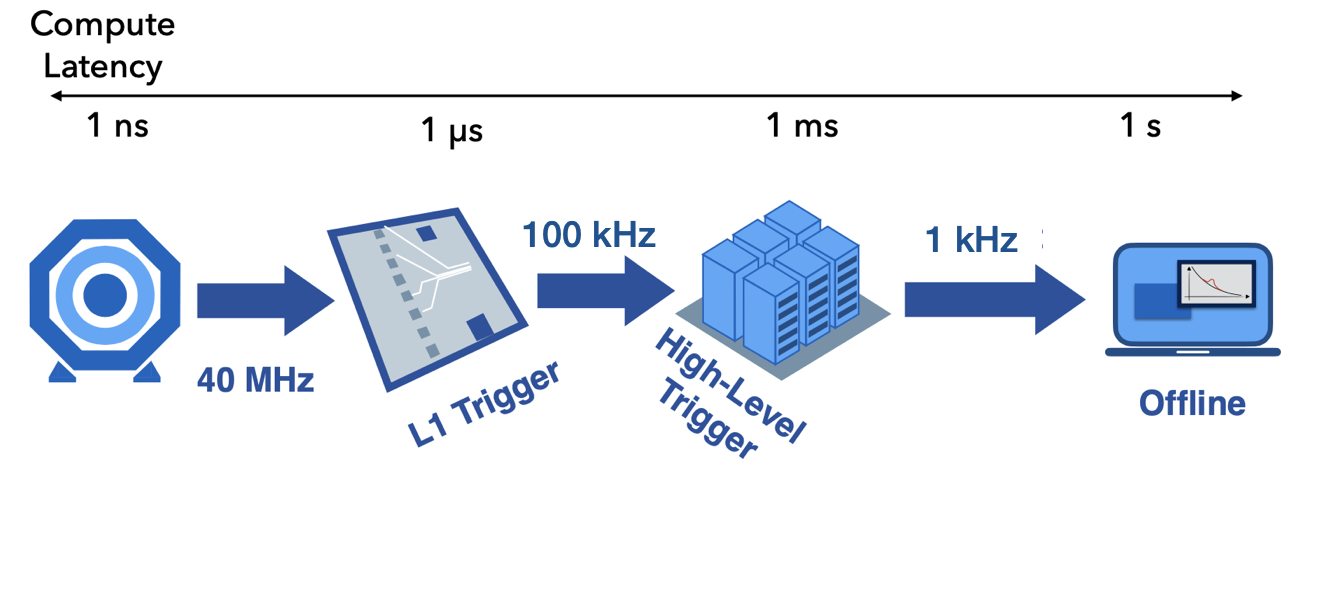
\includegraphics[width=\textwidth]{figures/atlas/trig-latency-graphic}
\caption{Illustration of the data acquisition chain -- a sequence of decisions in hardware (L1) and software (HLT) which determines which events get saved \cite{javier-iaifi-2} \cite{ATL-COM-DAQ-2014-054}.}
\label{fig:trig-latency}
\end{figure}

The first stage is the Level I (L1) trigger takes a very coarse view of the detector and has a $\mu s$ to decide whether to keep the event. This prohibits computationally expensive algorithms (such as tracking) being run, so L1 only looks at trigger objects using information from the calorimeter and muon systems.
Since these algorithms need to be very fast, they're implemented in hardware using field programmable gate arrays (FPGAs) before the electronic signals are read off of the detector.
It reduces the rate by almost three orders of magnitude (to 100 kHz) for sending the electronic signals off of the detector.
 

The second stage is High Level Trigger (HLT) is the software based trigger system, that implements an event reconstruction very similar to the offline algorithms. At this stage, tracking information is available, so \Pqb-tagging information can be used in the trigger decision (of particular importance for the HH $\rightarrow$ 4b analysis). 
There are several different ``trigger streams'' or combinations of selections applied to the trigger objects to collect datasets of interest to the diverse physics program.  Events passed from all of these trigger steams get saved at a rate of 1 kHz while data is being taken. 
%The estimate of the jet's energy is also much more accurate than it was at L1. 



%\begin{figure}
%\centering
%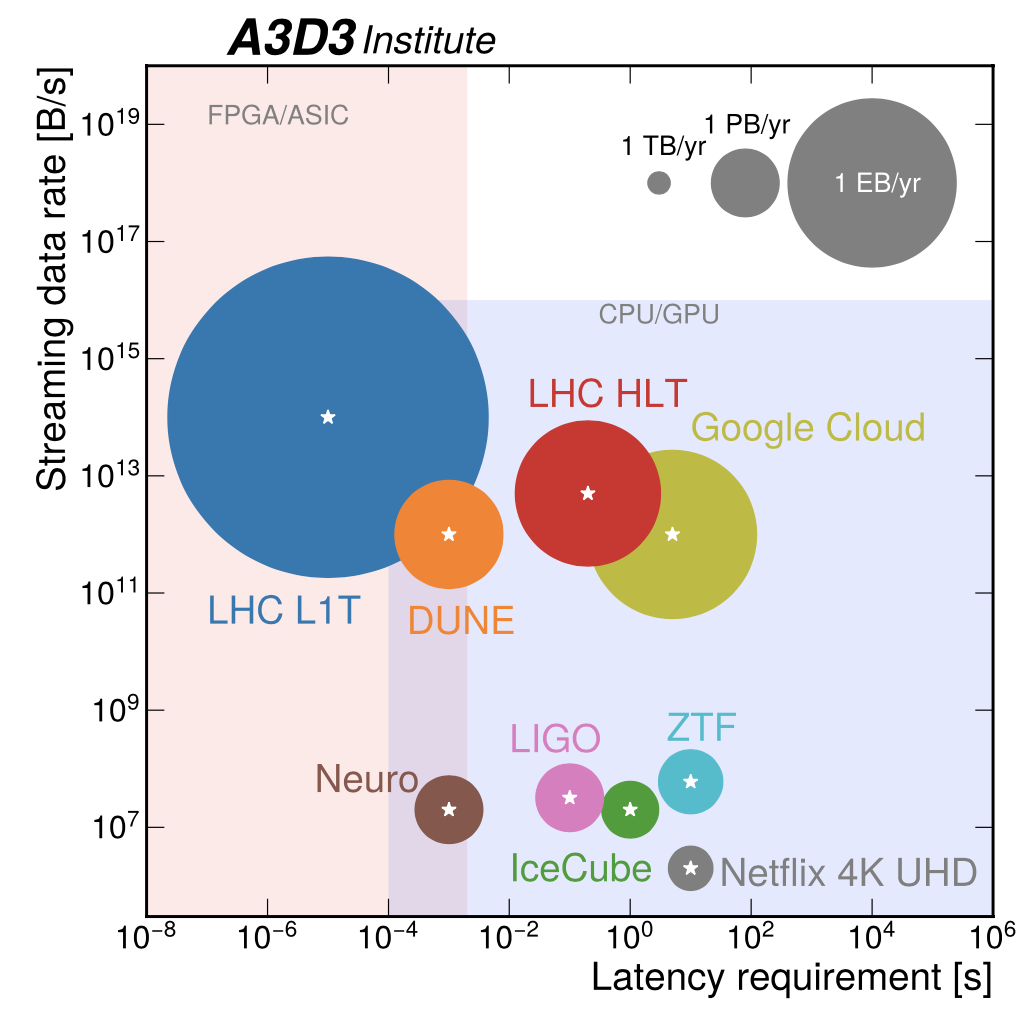
\includegraphics[width=.5\textwidth]{figures/atlas/dataset-sizes}
%\caption{\hl{If I include this, I'll have to find an original source to understand what everything means} \cite[javier-iaifi-2].}
%\label{fig:dataset-sizes}
%\end{figure}